%%%%%%%%%%%%%%%%%%%%%%%%%%%%%%%%%%%%%%%%%%%%%%%%%%%%%%%%%%%%%%%
% Welcome to the MAT320 Homework template on Overleaf -- just edit your
% LaTeX on the left, and we'll compile it for you on the right.
%%%%%%%%%%%%%%%%%%%%%%%%%%%%%%%%%%%%%%%%%%%%%%%%%%%%%%%%%%%%%%%
% --------------------------------------------------------------
% Based on a homework template by Dana Ernst.
% --------------------------------------------------------------
% This is all preamble stuff that you don't have to worry about.
% Head down to where it says "Start here"
% --------------------------------------------------------------

\documentclass[12pt]{article}

\usepackage{graphicx}
\graphicspath{{./images/}}
\usepackage{textcomp} % cent symbol, such as \textcent
\usepackage[margin=1in]{geometry} 
\usepackage{amsmath,amsthm,amssymb}
\usepackage{mathtools} % ceiling function
\DeclarePairedDelimiter{\ceil}{\lceil}{\rceil}
% https://tex.stackexchange.com/questions/146306/how-to-make-horizontal-lists
\usepackage[inline]{enumitem} % allows using letters in enumerate list environment

% source: https://stackoverflow.com/questions/3175105/inserting-code-in-this-latex-document-with-indentation

\usepackage{listings}
\usepackage{color}

\definecolor{dkgreen}{rgb}{0,0.6,0}
\definecolor{gray}{rgb}{0.5,0.5,0.5}
\definecolor{mauve}{rgb}{0.58,0,0.82}

\lstset{frame=tb,
	language=VHDL, % language for code listing
	aboveskip=3mm,
	belowskip=3mm,
	showstringspaces=false,
	columns=flexible,
	basicstyle={\small\ttfamily},
	numbers=none,
	numberstyle=\tiny\color{gray},
	keywordstyle=\color{blue},
	commentstyle=\color{dkgreen},
	stringstyle=\color{mauve},
	breaklines=true,
	breakatwhitespace=true,
	tabsize=4
}

\newcommand{\N}{\mathbb{N}}
\newcommand{\Z}{\mathbb{Z}}

\newenvironment{ex}[2][Exercise]{\begin{trivlist}
		\item[\hskip \labelsep {\bfseries #1}\hskip \labelsep {\bfseries #2.}]}{\end{trivlist}}

\newenvironment{sol}[1][Solution]{\begin{trivlist}
		\item[\hskip \labelsep {\bfseries #1:}]}{\end{trivlist}}


\begin{document}

% --------------------------------------------------------------
%                         Start here
% --------------------------------------------------------------

\noindent Sergio Garcia Tapia \hfill

\noindent{\small Digital Design and Computer Architecture: RISC-V, by
Sarah and David Harris} \hfill

\noindent{\small Chapter 4: Hardware Description Languages} \hfill 

\noindent\today

The following exercises may be done using your favorite HDL. If you have a
simulator available, test your design. Print the waveforms and explain
how they prove that it works. If you have a synthesizer available, synthesize
your code. Print the generated circuit diagram, and explain why it matches
your expectations.

\begin{ex}{4.1}
	Sketch a schematic of the circuit described by the following HDL code.
	Simplify the schematic so that it shows a minimum number of gates.
	\lstinputlisting[language={VHDL}]{./hdl/01-exercise1/exercise1.vhd}
\end{ex}

\begin{sol}
	The circuit has three inputs, $A,B,C$, and two outputs, $Y,Z$.
	Each output is defined by
	\begin{align*}
		Y&=ABC+AB\bar{C}+A\bar{B}C\\
		Z&=AB+\bar{A}\bar{B}
	\end{align*}
	We can simply $Y$ to:
	\begin{align*}
		Y&=AB\bar{C}+ABC+A\bar{B}C\\
		&=AB\bar{C}+ABC+ABC+A\bar{B}C\\
		&=AB+AC\\
		&=A(B+C)
	\end{align*}
	The sketch of the circuit is in Figure~\ref{04-01-circuit-sketch}.
	\begin{figure}
		\centering
		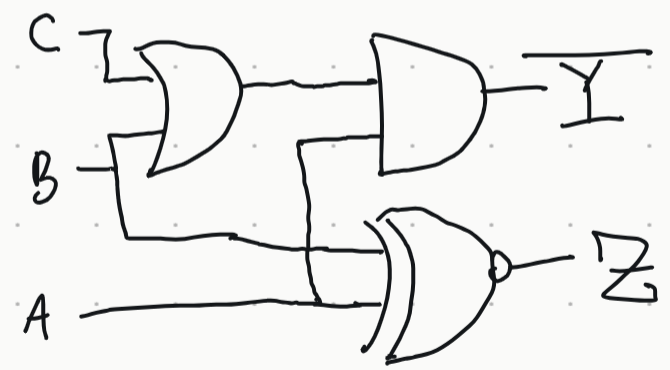
\includegraphics[width=0.3\textwidth]{04-01-circuit-sketch}
		\caption{Schematic sketch for Exercise 4-1}
		\label{04-01-circuit-sketch}
	\end{figure}
	The circuit synthesized by Quartus II is in Figure~\ref{04-01-synth-circuit}.
	\begin{figure}
		\centering
		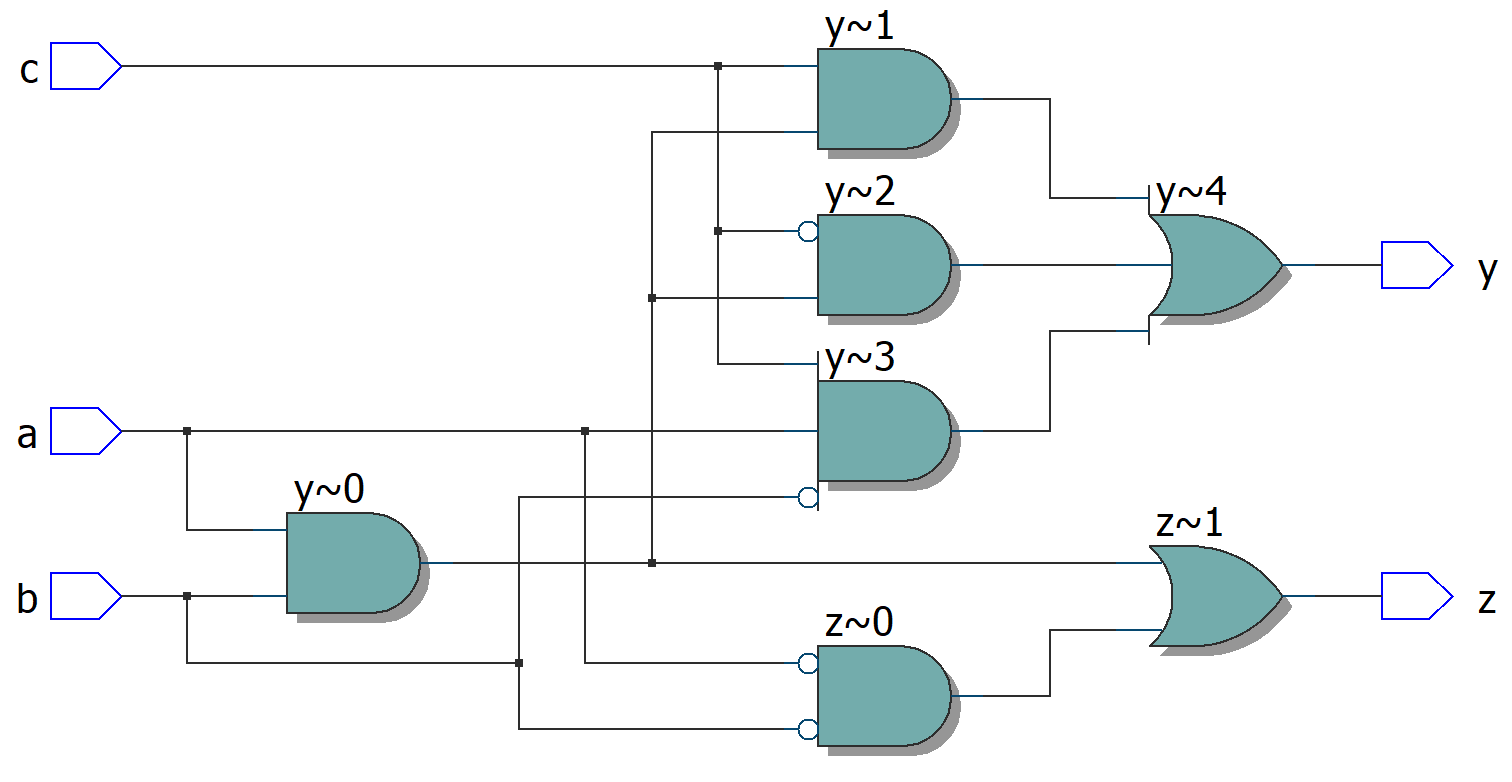
\includegraphics[width=0.5\textwidth]{04-01-synth-circuit}
		\caption{Synthesized Circuit by Quartus II for Exercise 4-1.}
		\label{04-01-synth-circuit}
	\end{figure}
\end{sol}

\begin{ex}{4.2}
	Sketch a schematic of the circuit described by the following HDL
	code. Simplify the schematic so that it shows a minimum number
	of gates.
	\lstinputlisting[language={VHDL}]{./hdl/02-exercise2/exercise2.vhd}
\end{ex}

\begin{sol}
	Note that the input is $A_{3:0}$ and the output is $Y_{1:0}$. Then $Y_1=A_0+A_1$ and
	$Y_0=A_0+A_2\bar{A_1}$. The sketch of the circuit is in Figure~\ref{04-02-circuit-sketch}.
	\begin{figure}
		\centering
		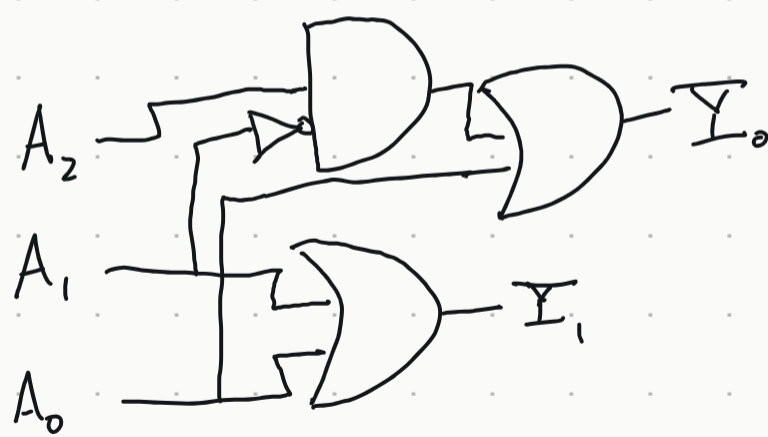
\includegraphics[width=0.4\textwidth]{04-02-circuit-sketch}
		\caption{Schematic sketch for Exercise 4-2}
		\label{04-02-circuit-sketch}
	\end{figure}
		The circuit synthesized by Quartus II is in Figure~\ref{04-01-synth-circuit}.
	\begin{figure}
		\centering
		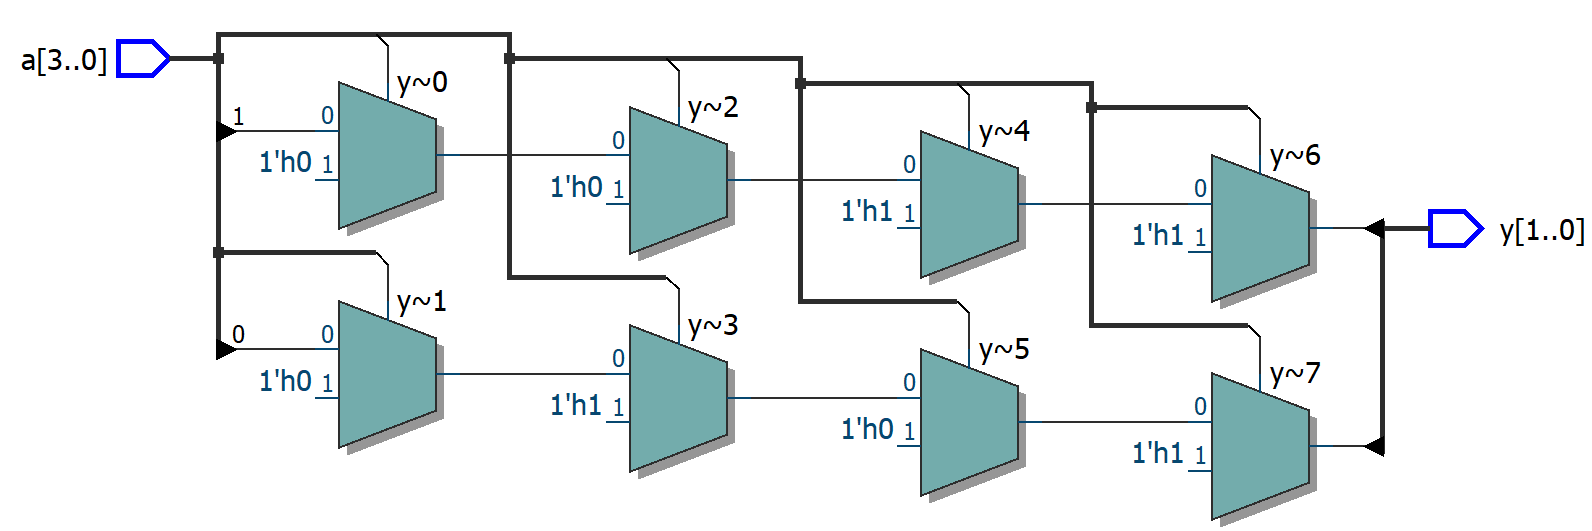
\includegraphics[width=0.8 \textwidth]{04-02-synth-circuit}
		\caption{Synthesized Circuit by Quartus II for Exercise 4-2.}
		\label{04-02-synth-circuit}
	\end{figure}
\end{sol}

\begin{ex}{4.3}
	Write an HDL module that computes a four-input XOR function. The input is $a_{3:0}$ and
	the output is $y$.
\end{ex}

\begin{sol}
	See the following listing, which can be found at
	\texttt{./hdl/03-04-xor4/xor4.vhd}:
	\lstinputlisting[language={VHDL}]{./hdl/03-04-xor4/xor4.vhd}
\end{sol}

\begin{ex}{4.4}
	Write a self-checking testbench for Exercise 4.3. Create a test vector file containing all 16 cases. Simulate the circuit and show that it works. Introduce an error in the 
	test vector file and show that the testbench reports a mismatch.
\end{ex}

\begin{sol}
	 The 16 cases are given in \texttt{./hdl/03-04-xor4/testvectors.txt}, available in the
	 following listing:
	\lstinputlisting[language={}]{./hdl/03-04-xor4/testvectors.txt}
	The self-checking testbench is available in \texttt{./hdl/03\_04/tb\_xor4.vhd.},
	which is a light modification of HDL Example 4.39. Specifically, it changes
	the file path to \texttt{../../testvectors.txt}, and the component used from
	\texttt{sillyfunction} to \texttt{xor4}:
	\lstinputlisting[language={VHDL}]{./hdl/03-04-xor4/tb_xor4.vhd}
	By modifying the last entry in the \texttt{./hdl/03-04-xor4/testvectors.txt}
	so that it says \texttt{1111\_1} instead, an error is reported, since
	the 4-input XOR gate should output 0 if there is an even number of 1s
	or all 0s, but the modified vector expects a 1.
\end{sol}

\begin{ex}{4.5}
	Write an HDL module called \texttt{minority}. It receives three inputs \texttt{a}, \texttt{b}, and
	\texttt{c}. It produces one output, \texttt{y}, that is TRUE if at least two of the inputs
	are FALSE.
\end{ex}

\begin{sol}
	The truth table for the Boolean function is below:
	\begin{center}
		\begin{tabular}{ccc|c}
			$A$ & $B$ & $C$ & $Y$\\
			\hline
			0 & 0 & 0 & 1\\
			0 & 0 & 1 & 1\\
			0 & 1 & 0 & 1\\
			0 & 1 & 1 & 0\\
			1 & 0 & 0 & 1\\
			1 & 0 & 1 & 0\\
			1 & 1 & 0 & 0\\
			1 & 1 & 1 & 0\\
		\end{tabular}
	\end{center}
	From the table we are able to identify the minterms and write
	\[
	Y=\bar{A}\bar{B}\bar{C}+\bar{A}\bar{B}C+\bar{A}B\bar{C}+A\bar{B}\bar{C}
	\]
	Though we could reduce the equation via Karnaugh maps, we let the HDL program handle the reduction.
	The listing is below:
	\lstinputlisting[language={VHDL}]{./hdl/05-minority/minority.vhd}
	The synthesized circuit is given in Figure~\ref{04-05-minority-circuit-synth}
	\begin{figure}
		\centering
		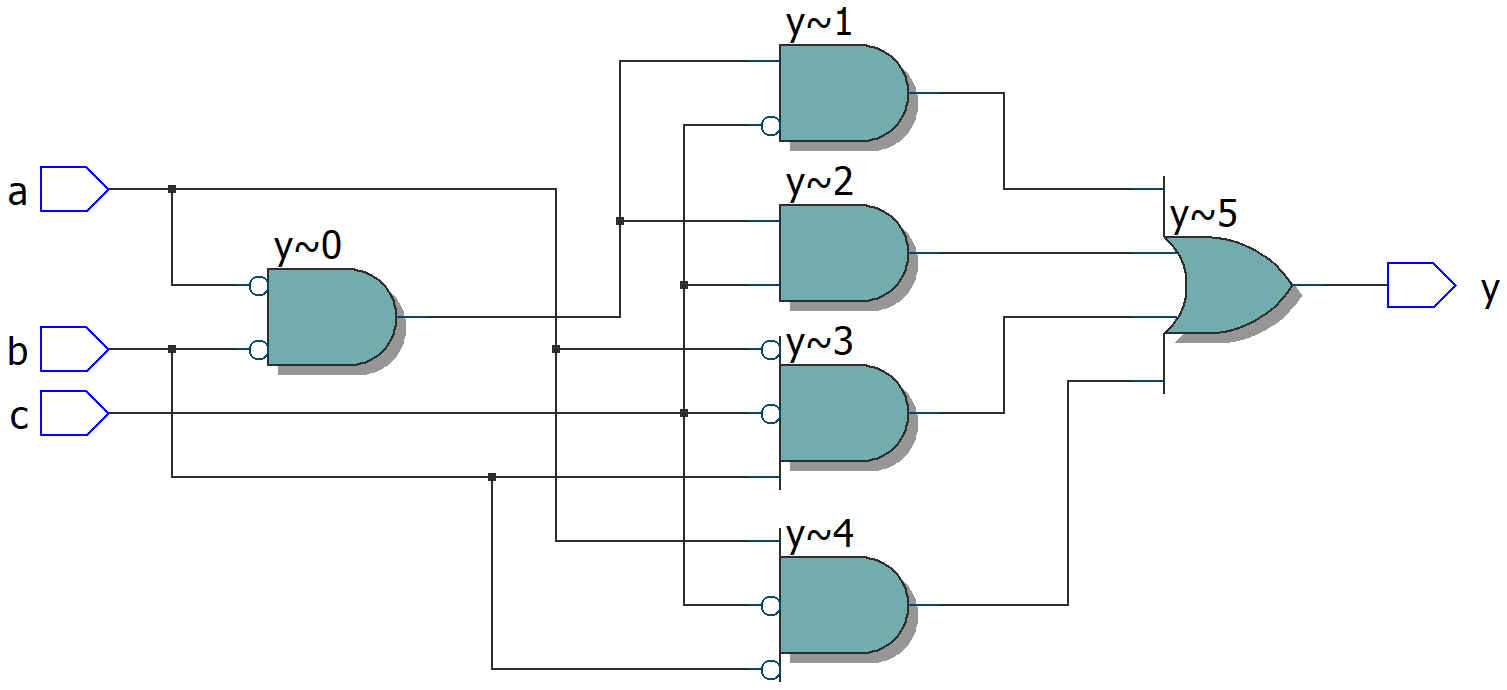
\includegraphics[width=0.5\textwidth]{04-05-minority-synth-circuit}
		\caption{Synthesized circuit for \texttt{minority} module in Exercise 4.5}
		\label{04-05-minority-circuit-synth}
	\end{figure}
	The truth table also forms the basis for the test vectors used in the test bench:
	\lstinputlisting[language={}]{./hdl/05-minority/testvectors.txt}
	Using a self-checking testbench adapted from HDL Example 4.39, the simulation is successful,
	so the module correctly models the boolean function.
\end{sol}

\begin{ex}{4.6}
	Write an HDL module for a hexadecimal seven-segment display decoder. The decoder should
	handle the digits A, B, C, D, E and F, as well as 0-9.
\end{ex}

\begin{sol}
	Figure~\ref{seven-segment-display-decoder} and Figure~\ref{seven-segment-display-digits}
	show the images from Chapter 2 for this circuit. Figure~\ref{04-06-seven-segment-display-hex-letters}
	shows the letters used in hexadecimal using seven segments. Notice that it uses
	lowercase $b$ and $d$, since their uppercase versions would be confused with $8$ and $0$,
	respectively.
	\begin{figure}
		\centering
		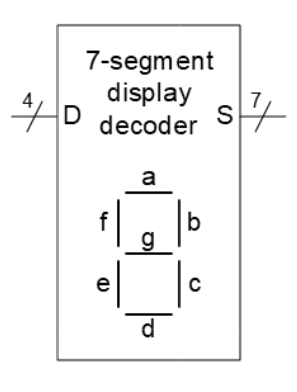
\includegraphics[width=0.3\textwidth]{seven-segment-display-decoder}
		\caption{Seven Segment Display Decoder Circuit}
		\label{seven-segment-display-decoder}
	\end{figure}
	\begin{figure}
		\centering
		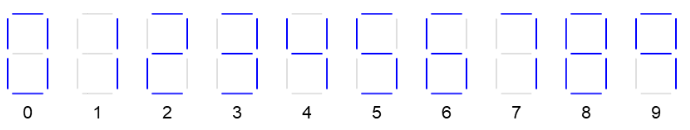
\includegraphics[width=0.7\textwidth]{seven-segment-display-digits}
		\caption{Seven Segment Display Digits}
		\label{seven-segment-display-digits}
	\end{figure}
	\begin{figure}
		\centering
		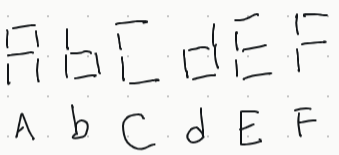
\includegraphics[width=0.7\textwidth]{04-06-seven-segment-display-hex-letters}
		\caption{Seven Segment Display Hex Letters}
		\label{04-06-seven-segment-display-hex-letters}
	\end{figure}
	The truth table is
	\begin{center}
		\begin{tabular}{c|ccccccc}
			$D_{3:0}$ & $S_a$ & $S_b$ & $S_c$ & $S_d$ & $S_e$ & $S_f$ & $S_g$\\
			\hline
			0000 & 1 & 1 & 1 & 1 & 1 & 1 & 0\\
			0001 & 0 & 1 & 1 & 0 & 0 & 0 & 0\\
			0010 & 1 & 1 & 0 & 1 & 1 & 0 & 1\\
			0011 & 1 & 1 & 1 & 1 & 0 & 0 & 1\\
			0100 & 0 & 1 & 1 & 0 & 0 & 1 & 1\\
			0101 & 1 & 0 & 1 & 1 & 0 & 1 & 1\\
			0110 & 1 & 0 & 1 & 1 & 1 & 1 & 1\\
			0111 & 1 & 1 & 1 & 0 & 0 & 0 & 0\\
			1000 & 1 & 1 & 1 & 1 & 1 & 1 & 1\\
			1001 & 1 & 1 & 1 & 0 & 0 & 1 & 1\\
			1010 & 1 & 1 & 1 & 0 & 1 & 1 & 1\\
			1011 & 0 & 0 & 1 & 1 & 1 & 1 & 1\\
			1100 & 1 & 0 & 0 & 1 & 1 & 1 & 0\\
			1101 & 0 & 1 & 1 & 1 & 1 & 0 & 1\\
			1110 & 1 & 0 & 0 & 1 & 1 & 1 & 1\\
			1111 & 1 & 0 & 0 & 0 & 1 & 1 & 1\\
		\end{tabular}
	\end{center}
	It is not necessary to create Boolean equations and write out the minterms. The following
	code listing shows the implementation:
	\lstinputlisting[language={VHDL}]{./hdl/06-seven-segment-hex-decoder/seven_segment_hex_decoder.vhd}
\end{sol}

\begin{ex}{4.7}
	Write a self-checking testbench for Exercise 4.6. Create a test vector file containing all
	16 cases. Simulate the circuit and show that it works. Introduce an error in the test vector
	file and show that the testbench reports a mismatch.
\end{ex}

\begin{sol}
	We can use the following vector file, \texttt{testvectors.txt}:
	\lstinputlisting[language={}]{./hdl/06-seven-segment-hex-decoder/testvectors.txt}
	The code listing below, \texttt{06-seven-segment-hex-decoder/tb\_seven\_segment\_hex\_decoder.vhd} is the testbench module:
	\lstinputlisting[language={VHDL}]{./hdl/06-seven-segment-hex-decoder/tb_seven_segment_hex_decoder.vhd}
\end{sol}

\begin{ex}{4.8}
	Write an 8:1 multiplexer module called \texttt{mux8} with inputs \texttt{s$_{2:0}$}, \texttt{d0},
	\texttt{d1},\texttt{d2},\texttt{d3},\texttt{d4},\texttt{d5},\texttt{d6},\texttt{d7}, and output
	\texttt{y}.
\end{ex}

\begin{sol}
	The following code listing implements \texttt{mux8} with generics,
	where the inputs and outputs are vectors of any given length.
	\lstinputlisting{./hdl/08-mux8/mux8.vhd}
\end{sol}

\begin{ex}{4.9}
	Write a structural module to compute the logic function
	$Y=A\bar{B}+\bar{B}\bar{C}+\bar{A}BC$ using multiplexer logic.
	Use the 8:1 multiplexer from Exercise 4.8.
\end{ex}

\begin{sol}
	Recall, as discussed in Section 2.8.1, that any $2^{N}$-input
	multiplexer can be programmed to perform any $N$-input multiplexer.
	Since $Y$ has 3 inputs, we can use an 8-input multiplexer, which
	is precisely \texttt{mux8} from the previous exercise.
	We begin by creating the boolean table:
	\begin{center}
		\begin{tabular}{ccc|c}
			$A$ & $B$ & $C$ & $Y$\\
			\hline
			0 & 0 & 0 & 1\\
			0 & 0 & 1 & 0\\
			0 & 1 & 0 & 0\\
			0 & 1 & 1 & 1\\
			1 & 0 & 0 & 1\\
			1 & 0 & 1 & 1\\
			1 & 1 & 0 & 0\\
			1 & 1 & 1 & 0
		\end{tabular}
	\end{center}
	It serves as the basis for the test vector file, as well as
	the HDL module, listed in \texttt{./hdl/09-structmodule/structmodule.vhd}
	\lstinputlisting{./hdl/09-structmodule/structmodule.vhd}
\end{sol}

\begin{ex}{4.10}
	Repeat Exercise 4.9 using a 4:1 multiplexer and as many NOT gates
	as you need.
\end{ex}

\begin{sol}
	Section 2.8.1 mentions its possible to represent any $N$-input
	logic function with a $2^{N-1}$ input multiplexer. We eliminate $C$
	and express the output of $Y=A\bar{B}+\bar{B}\bar{C}+\bar{A}BC$ in terms of $C$:
	\begin{center}
		\begin{tabular}{cc|c}
			$A$ & $B$ & $Y$\\
			\hline
			0 & 0 & $\overline{C}$\\
			0 & 1 & $C$\\
			1 & 0 & 1\\
			1 & 1 & 0\\   
		\end{tabular} 
	\end{center}
	The \texttt{mux4} is given below in \texttt{./hdl/10-structmodulemux4/mux4.vhd}
	\lstinputlisting{./hdl/10-structmodulemux4/mux4.vhd}
	The boolean function is implemented in the module in
	\texttt{./hdl/10-structmodulemux4/structmodule.vhd}
	\lstinputlisting{./hdl/10-structmodulemux4/structmodule.vhd}
\end{sol}

\begin{ex}{4.12}
	Write an HDL module for an eight-input priority circuit.
\end{ex}

\begin{sol}
	See the code listing for \texttt{./hdl/12-priority8/priority8.vhd} below:
	\lstinputlisting{./hdl/12-priority8/priority8.vhd}
\end{sol}

\begin{ex}{4.13}
	Write an HDL module for a 2:4 decoder.
\end{ex}

\begin{sol}
	A 2-input 4-output decoder chooses one of its 4 outputs according to
	the given input combination. See the table below:
	\begin{center}
		\begin{tabular}{cc|cccc}
			$A_1$ & $A_0$ & $Y_3$ & $Y_2$ & $Y_1$ & $Y_0$\\
			\hline
			0 & 0 & 0 & 0 & 0 & 1\\
			0 & 1 & 0 & 0 & 1 & 0\\
			1 & 0 & 0 & 1 & 0 & 0\\
			1 & 1 & 1 & 0 & 0 & 0\\
		\end{tabular}
	\end{center}
	See the code listing for \texttt{./hdl/13-decoder2\_4/decoder2\_4.vhd}.
	\lstinputlisting{./hdl/13-decoder2_4/decoder2_4.vhd}
\end{sol}

\begin{ex}{4.14}
	Write an HDL module for a 6:64 decoder using three instances of
	the 2:4 decoders from Exercise 4.13 and a bunch of three-input AND gates.
\end{ex}

\begin{sol}
	Let the input be $D_{5:0}$, and split them into three 2-bit groups: $D_{5:4}$, $D_{3:2}$, and $D_{1:0}$.
	Each group will be fed into a separate decoder, each producing outputs
	$A_{3:0}$, $B_{3:0}$, and $C_{3:0}$ as follows:
	\begin{align*}
		D_{5:4} & \to A_{3:0}\\
		D_{3:2} & \to B_{3:0}\\
		D_{1:0} & \to C_{3:0}
	\end{align*}
	Then, we'll have 64 different three-input AND gates. Letting $0\leq i, j, k \leq 3$,
	we'll have AND gate for all 64 combinations of $Y_m=A_iB_jC_k$, where $m=16i+4j+k$.
	For example, if $D_{5:0}$ is all zeroes, then $D_{5:4}, D_{3:2},D_{1:0}$ are also all zeroes,
	so that $A_0=B_0=C_0=1$. Since $Y_0=A_0B_0C_0$, it follows that $Y_0$, as required. If,
	on the other hand, any bit is 1, then one of $A_0$, $B_0$, or $C_0$ will be 0,
	so the output $Y_0$ becomes 0, as required. All other cases are justified similarly.
	
	The following code listing,
	\texttt{./hdl/14-decoder6\_64/decoder6\_64.vhd}, uses \texttt{generate} to loop and create
	all combinations.
	\lstinputlisting{./hdl/14-decoder6_64/decoder6_64.vhd}
	
	The following code listing, \texttt{./hdl/14-decoder6\_64/tb\_decoder6\_64.vhd} is a
	self-checking test bench that verifies it works
	\lstinputlisting{./hdl/14-decoder6_64/tb_decoder6_64.vhd}
\end{sol}

\begin{ex}{4.16}
	Write an HDL module that implements the circuit from Exercise 2.26. See Figure~{04-16-circuit}.
	\begin{figure}
		\centering
		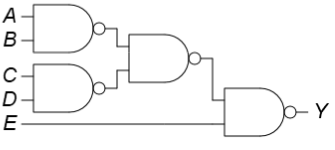
\includegraphics{04-16-circuit}
		\caption{Circuit from Exercise 2.26 for Exercise 4.16}
		\label{04-16-circuit}
	\end{figure}
\end{ex}

\begin{sol}
	See code listing \texttt{./hdl/16-exercise2\_26/exercise2\_26.vhd}:
	\lstinputlisting{./hdl/16-exercise2_26/exercise2_26.vhd}
\end{sol}

\begin{ex}{4.18}
	Write an HDL module that implements the logic from Exercise 2.28. Pay careful attention
	to how you handle don't cares. See Figure~\ref{04-18-truthtable}.
	\begin{figure}
		\centering
		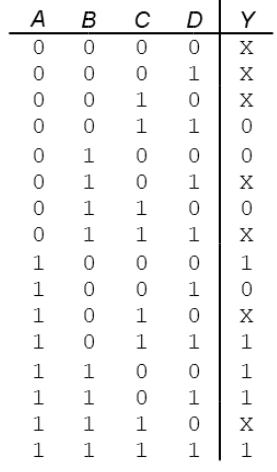
\includegraphics[width=0.3\textwidth]{04-18-truthtable}
		\caption{Truth table for Exercise 4.18}
		\label{04-18-truthtable}
	\end{figure}
\end{ex}

\begin{sol}
	We can make it so that the input combinations that lead to don't cares yield 0.
	See code listing \texttt{./hdl/18-exercise2\_28/exercise2\_26.vhd}:
	\lstinputlisting{./hdl/18-exercise2_28/exercise2_28.vhd}
\end{sol}

\begin{ex}{4.19}
	Write an HDL module that implements the functions from Exercise 2.35.
\end{ex}

\begin{sol}
	The specification is that we have an input $A_{3:0}$, representing the numbers 0 through 15.
	There are two outputs: $P$ is TRUE if the number is prime, and $D$ is true if the number is
	divisible by 3. The truth table below shows the function inputs and outputs:
	\begin{center}
		\begin{tabular}{cccc|cc}
			$A_3$ & $A_2$ & $A_1$ & $A_0$ & $P$ & $D$\\
			\hline
			0 & 0 & 0 & 0 & 0 & 1\\
			0 & 0 & 0 & 1 & 0 & 0\\
			0 & 0 & 1 & 0 & 1 & 0\\
			0 & 0 & 1 & 1 & 1 & 1\\
			0 & 1 & 0 & 0 & 0 & 0\\
			0 & 1 & 0 & 1 & 1 & 0\\
			0 & 1 & 1 & 0 & 0 & 1\\
			0 & 1 & 1 & 1 & 1 & 0\\
			1 & 0 & 0 & 0 & 0 & 0\\ %8
			1 & 0 & 0 & 1 & 0 & 1\\ %9
			1 & 0 & 1 & 0 & 0 & 0\\ %10
			1 & 0 & 1 & 1 & 1 & 0\\ %11
			1 & 1 & 0 & 0 & 0 & 1\\ %12
			1 & 1 & 0 & 1 & 1 & 0\\ %13
			1 & 1 & 1 & 0 & 0 & 0\\ %14
			1 & 1 & 1 & 1 & 0 & 1\\ %15
		\end{tabular}
	\end{center}
	
	See code listing \texttt{./hdl/19-exercise2\_35/exercise2\_35.vhd}:
	\lstinputlisting{./hdl/19-exercise2_35/exercise2_35.vhd}
\end{sol}

\begin{ex}{4.24}
	Sketch the state transition diagram for the FSM described by the following HDL code.
	\begin{lstlisting}
library IEEE; use IEEE.STD_LOGIC_1164.all;

entity fsm2 is
  port(clk, reset: in  STD_LOGIC;
       a, b:       in  STD_LOGIC;
       y:          out STD_LOGIC);
end;

architecture synth of fsm2 is
  type statetype is (S0, S1, S2, S3);
  signal state, nextstate: statetype;
begin
  process(clk, reset) begin
    if reset then state <= S0;
    elsif rising_edge(clk) then
      state <= nextstate;
    end if;
  end process;
  
  process(all) begin
    case state is
      when S0 => if (a xor b) then
                       nextstate <= S1;
                 else  nextstate <= S0;
                 end if;
      when S1 => if (a and b) then
      				   nextstate <= S2;
      		     else  nextstate <= S0;
      			 end if;
      when S2 => if (a or b) then
					   nextstate <= S3;
				 else  nextstate <= S0;
				 end if;
      when S3 => if (a or b) then
				 	   nextstate <= S3;
				 else  nextstate <= S0;
				 end if;
  end process;
  
  y <= '1' when((state = S1) or (state = S2))
       else '0';
end;
	\end{lstlisting}
\end{ex}

\begin{sol}
	This is a Moore state machine. See Figure~\ref{04-24-state-transition-diagram}.
	\begin{figure}
		\centering
		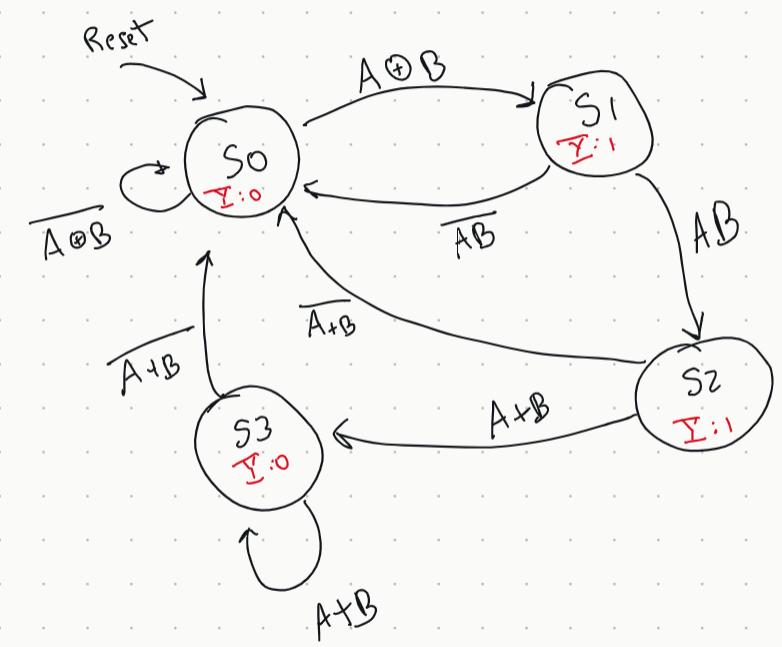
\includegraphics[width=0.5\textwidth]{04-24-state-transition-diagram}
		\caption{State Transition Diagram for Exercise 4.24}
		\label{04-24-state-transition-diagram}
	\end{figure}
\end{sol}

\begin{ex}{4.25}
	Sketch the state transition diagram for the FSM described by the following HDL code.
	An FSM of this nature is used in a branch predictor on some microprocessors.
	\begin{lstlisting}
library IEEE; use IEEE.STD_LOGIC_1164.all;

entity fsm1 is
  port(clk, reset:   in STD_LOGIC;
       taken, back:  in STD_LOGIC;
       predicttaken: in STD_LOGIC);
end;

architecture synth of fsm1 is
  type statetype is (S0, S1, S2, S3, S4);
  signal state, nextstate: statetype;
begin
  process(clk, reset) begin
    if reset then state <= S2;
    elsif rising_edge(clk) then
      state <= nextstate;
    end if;
  end process;
  
  process(all) begin
    case state is
      when S0 => if taken then
      				  nextstate <= S1;
      			 else nextstate <= S0;
      			 end if;
      when S1 => if taken then
       				  nextstate <= S2;
       			 else nextstate <= S0;
       			 end if;
      when S2 => if taken then
       				  nextstate <= S3;
       			 else nextstate <= S1;
       			 end if;
      when S3 => if taken then
        			  nextstate <= S4;
        		 else nextstate <= S2;
        		 end if;
      when S4 => if taken then
           			  nextstate <= S4;
           		 else nextstate <= S3;
           		 end if;
      when others =>  nextstate <= S2;
    end case;
  end process;
  
  -- output logic
  predicttaken <= '1' when
                  ((state = S4) or (state = S3) or
                  (state = S2 and back = '1'))
end;
	\end{lstlisting}
\end{ex}

\begin{sol}
	This is a Mealy state machine. See Figure~\ref{04-25-state-transition-diagram}.
	\begin{figure}
		\centering
		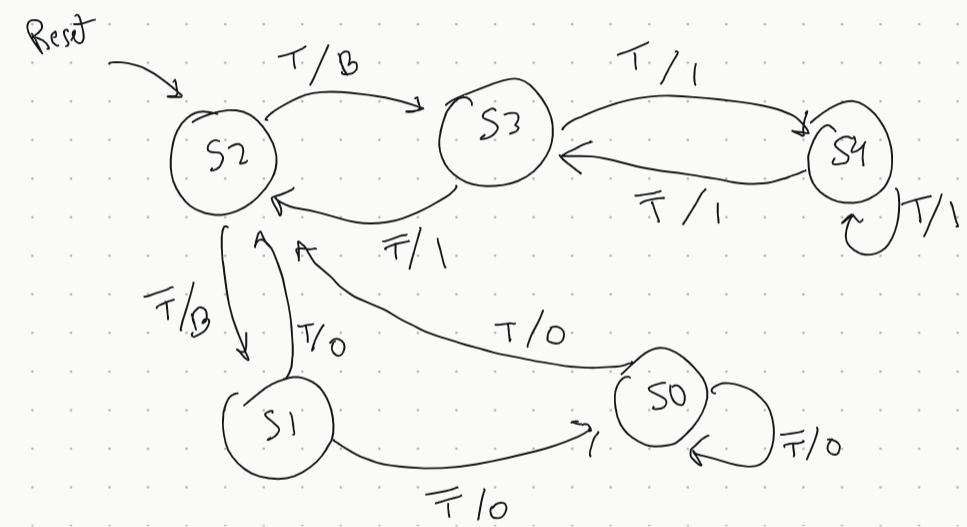
\includegraphics[width=0.6\textwidth]{04-25-state-transition-diagram}
		\caption{State Transition Diagram for Exercise 4.25}
		\label{04-25-state-transition-diagram}
	\end{figure}
\end{sol}

\begin{ex}{4.26}
	Write an HDL module for an SR latch.
\end{ex}

\begin{sol}
	See code listing \texttt{./hdl/26-sr\_latch/sr\_latch.vhd}
	\lstinputlisting{./hdl/26-sr_latch/sr_latch.vhd}
\end{sol}

\begin{ex}{4.27}
	Write an HDL module for a \emph{JK flip-flop}. The flip-flop has inputs \emph{CLK}, \emph{J}, and
	\emph{K}, and output \emph{Q}. On the rising edge of the clock, \emph{Q} keeps its old value if
	$J=K=0$. It sets $Q$ to 1 if $J=1$, resets $Q$ to 0 if $K=1$, and inverts $Q$ if $J=K=1$.
\end{ex}

\begin{sol}
	See code listing \texttt{./hdl/27-jk\_ff/jk\_ff.vhd}:
	\lstinputlisting{./hdl/27-jk_ff/jk_ff.vhd}
\end{sol}

\begin{ex}{4.29}
	Write an HDL module for the traffic light controller from Section 3.4.1.
\end{ex}

\begin{sol}
	See code listing \texttt{./hdl/29-traffic\_light/traffic\_light.vhd}
	\lstinputlisting{./hdl/29-traffic_light/traffic_light.vhd}
\end{sol}

\begin{ex}{4.30}
	Write HDL modules for the factored parade mode traffic light controller
	from Example 3.8. The modules should be called \texttt{controller},
	\texttt{mode}, and \texttt{lights}, and they should have the inputs
	and outputs shown in Figure~\ref{04-30-factored-traffic-fsm-design}.
	See the state transition diagram in Figure~\ref{04-30-factored-transition-diagrams}.
	\begin{figure}
		\centering
		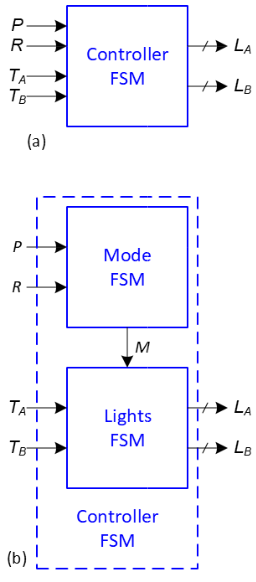
\includegraphics[width=0.2\textwidth]{04-30-factored-traffic-fsm-design}
		\caption{Factored Traffic Light State Machine Design for Exercise 4.30}
		\label{04-30-factored-traffic-fsm-design}
	\end{figure}
	\begin{figure}
	\centering
	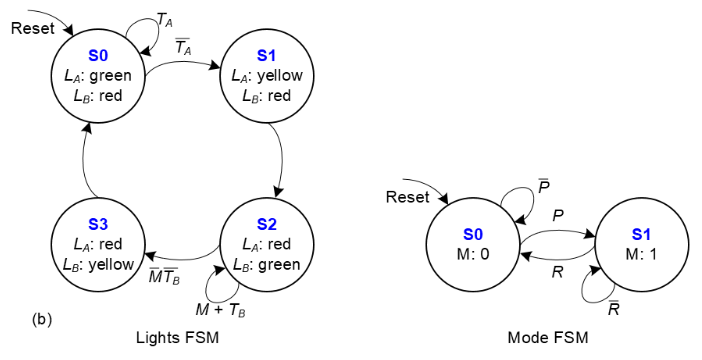
\includegraphics[width=0.7\textwidth]{04-30-factored-transition-diagrams}
	\caption{Factored Traffic Light State Transition Diagram for Exercise 4.30}
	\label{04-30-factored-transition-diagrams}
\end{figure}
\end{ex}

\begin{sol}
	The \texttt{mode} module is in listing \texttt{./hdl/30-traffic\_fsm\_factored/mode.vhd}:
	\lstinputlisting{./hdl/30-traffic_fsm_factored/mode.vhd}:
	
	The \texttt{lights} module is in listing \texttt{./hdl/30-traffic\_fsm\_factored/lights.vhd}:
	\lstinputlisting{./hdl/30-traffic_fsm_factored/lights.vhd}:
	
	The \texttt{controller} module is in listing \texttt{./hdl/30-traffic\_fsm\_factored/controller.vhd}:
	\lstinputlisting{./hdl/30-traffic_fsm_factored/controller.vhd}:
\end{sol}

\begin{ex}{4.31}
	Write an HDL describing the circuit in Figure~\ref{}. 
\end{ex}

\begin{sol}
	See code listing \texttt{./hdl/31-exercise31/exercise31.vhd}:
	\lstinputlisting{./hdl/31-exercise31/exercise31.vhd}
\end{sol}

\end{document}